\chapter{Upgrading the MEGA65}

\section{How a MEGA65 Can Be Upgraded}
\label{cha:cores}

The MEGA65 platform consists of three major components:

\begin{enumerate}
  \item The {\bf MEGA65 core},\index{Core} a description of the chipset to run on the FPGA
  \item The {\bf ROM},\index{ROM} code that defines the Commodore-style operating system (KERNAL) and BASIC
  \item {\bf System software} for features such as the Freezer menu\index{Freezer menu}
\end{enumerate}

You can upgrade these components as new releases are published. You can also replace one or more of these components individually. In the case of the core and ROM, you can even have multiple versions installed simultaneously and switch between them. For example, instead of the latest MEGA65 ROM, you can switch to the original Commodore 65 prototype ROM. Or, you could switch to another core that causes your MEGA65 hardware to behave like a different computer entirely, such as a Commodore 64 or a ZX Spectrum.

The ROM and system software are files that reside on the SD card, and upgrading them is as simple as replacing the files. To upgrade the core, you use a process to install a core file into the MEGA65's core flash memory. This chapter describes this process.

\subsection{What is a Core?}
\index{Core!definition}

The MEGA65 hardware architecture is based on a versatile chip called a ``Field Programmable Gate Array,'' or FPGA.\index{Field Programmable Gate Array (FPGA)} This is a special kind of computer chip that can be programmed to impersonate other chips. It does this by configuring a giant array of logic gates to reproduce circuits. FPGAs are not an emulation, but an electronic re-creation of other chips. FPGA code is sometimes referred to as {\em firmware,} a term you may recognize from modern computers and other devices.

Your MEGA65 was programmed at the factory to re-create a chipset based on the original Commodore 65, designed by the MEGA65 team. You can re-program the MEGA65 FPGA to upgrade to new versions of the MEGA65 chipset, or to replace the chipset with that of an entirely different computer!

Each possible chipset is known as a {\em core}. The MEGA65 can store up to eight cores, and you can switch between these cores by accessing a menu when you switch on the computer. You can also use this menu to load a new core from a file on the SD card, a process known as {\em flashing}.

Members of the MEGA65 community have made several useful and fun alternate cores for the FPGA hardware. \href{https://github.com/MJoergen/C64MEGA65}{{\em C64 for MEGA65}} by MJoergen and sy2002 re-creates the original Commodore 64 computer with a high degree of accuracy, perfect for running Commodore 64 games, demos, and applications. Other cores re-create the ZX Spectrum, the Game Boy, and even the original Galaga arcade machine hardware. The MEGA65's FPGA is powerful enough to re-create nearly all 8-bit home computers, and likely some 16-bit computers and consoles such as the Commodore Amiga. The MEGA65 hardware design, board layout, FPGA core, and other information are all available for free under various open-source licenses, so anyone is free to create other cores for the MEGA65 hardware.

\section{Determining the Versions of Things}
\label{sec:versions}

All components of the MEGA65 platform have a version identifier. The MEGA65 can display the version identifiers for all of its components using the MEGA65 Information utility.\index{MEGA65 Information Utility}

To open the MEGA65 Information utility:

\begin{enumerate}
  \item Switch on the MEGA65, and allow it to boot to BASIC.
  \item Open the Freezer:\index{Freezer menu} press and hold \widekey{RESTORE} for one second then release it.
  \item Press \specialkey{HELP}. The MEGA65 Information utility will open.
\end{enumerate}

\begin{center}
  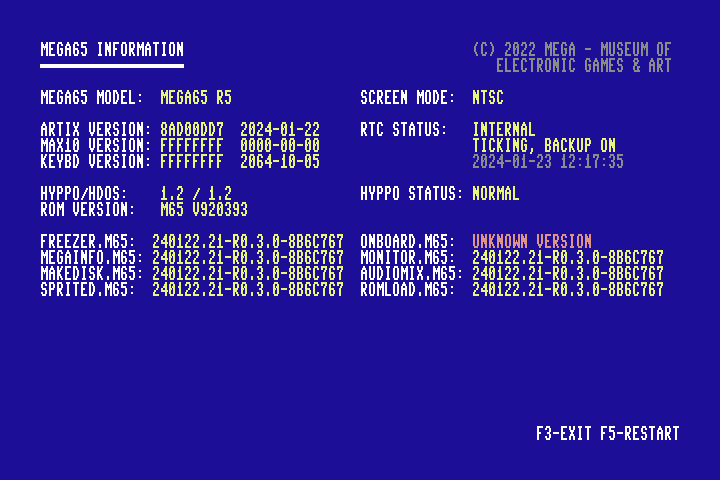
\includegraphics[width=0.7\linewidth]{images/megainfo.png}
\end{center}

Take note of these version identifiers:
\nopagebreak
\begin{center}
\setlength{\tabcolsep}{1mm}
\begin{tabularx}{\textwidth}{|X|p{7cm}|}
  \hline
  {\bf Label and Example} & {\bf Description} \\
  \hline
  MEGA65 Model\newline {\tt MEGA65 R6} & The revision of the hardware. You need to know this when downloading new core files. \\
  \hline
  Artix Version\index{Core!Version}\newline {\tt 8AD00DD7 2024-01-22} & The currently running MEGA65 core. This is a string of eight letters and numbers, and also a build date. \\
  \hline
  ROM Version\index{ROM!Version}\newline {\tt M65 V920393} & The currently running ROM. For MEGA65 ROMs, this is a sequential number, with larger numbers representing newer releases. \\
  \hline
  System files (.M65)\newline {\tt 240122.21-R0.3.0-8B6C767} & Each of the system software files has its own version identifier. Typically, you do not need to know these: you will upgrade these along with each core. The identifier is similar to the core version, but does not always match the currently running core. \\
  \hline
\end{tabularx}
\end{center}

Press \specialkey{F3} to exit to the Freezer, then \specialkey{F3} again to exit to BASIC.

Each core has a separate version for each hardware revision. As of the year 2024, the production models of the MEGA65 have used two different main board revisions, known as ``R3'' (more specifically ``R3A'') and ``R6.''\footnote{The MEGA65 ``DevKit'' model sold in the year 2020 is revision ``R3.'' It is also possible to run the MEGA65 core on certain FPGA development boards, with a separate version of the core file for each.}\index{Hardware revisions}

The MEGA65 core is available for all hardware revisions. If you are installing an alternate core and it is not available for your hardware revision, contact the author of the core.

\section{Obtaining the Latest Files}

You can download the latest MEGA65 core, ROM, and system software from the MEGA65 Filehost website.\index{Filehost website} Due to distribution restrictions for the Commodore 65 ROM code, some files require a Filehost account registered to a MEGA65 owner to access. All owners of the MEGA65 have a license to all versions of this ROM code.\footnote{There is a procedure for non-owners to get the latest MEGA65 ROM, such as to use with the \href{https://github.lgb.hu/xemu/}{Xemu MEGA65 emulator}. This involves downloading \href{https://www.c64forever.com/}{C64 Forever Free Express Edition} from Cloanto, extracting the original Commodore 65 prototype ROM file, then using a tool to apply a patch that you can download from Filehost. The full process is described in the following article: \url{https://mega65.org/rom-faq}}

Visit the following URL in your web browser:

\url{https://files.mega65.org}

\begin{center}
  \fbox{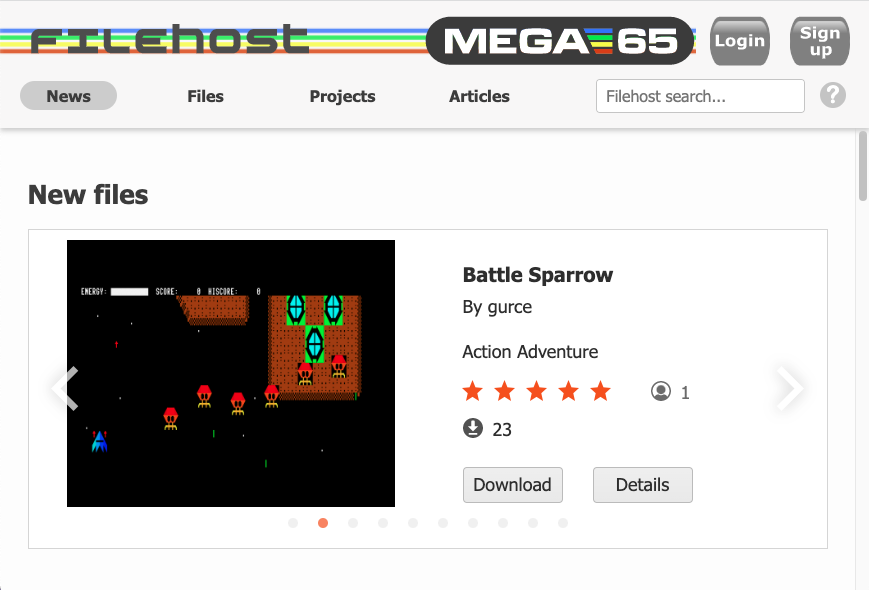
\includegraphics[width=0.7\linewidth]{images/filehost_notsignedin.png}}
\end{center}

To register a Filehost account with your owner code:

\begin{enumerate}
  \item Visit \href{https://files.mega65.org}{the Filehost website}. Click ``Sign Up.'' Follow the prompts to create an account.
  \item Locate your owner code.\index{Owner Code} This is a code printed on a piece of paper that was included with your MEGA65 (possibly inserted into this manual). It looks something like this: {\tt 123-ABC-456}
  \item Click the user icon in the upper-right corner of the Filehost screen. In the pop-up menu, select ``Redeem Code.'' Enter your owner code as prompted.
\end{enumerate}

\begin{center}
  \fbox{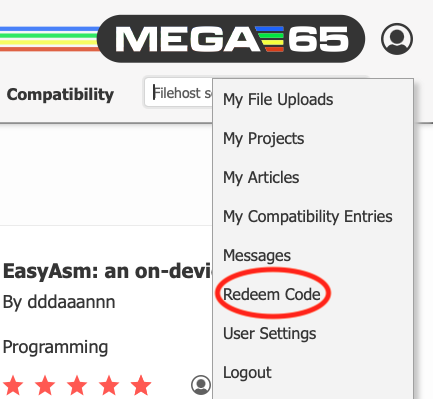
\includegraphics[width=0.4\linewidth]{images/filehost_redeemmenu.png}}
\end{center}

To download the latest release package:

\begin{enumerate}
  \item Click the ``Files'' tab of the Filehost website.
  \item In the search box on the left-hand side, type: ``release'' The list will update to show only files with that word in the title.
  \item Locate the entry named, ``MEGA65 Core Release Package (mega65r6) incl. ROM,'' where ``mega65r6'' matches your hardware revision. (To confirm your hardware revision, open the Freezer menu, then press \specialkey{Help}.)
  \item Click the entry. Confirm that this release package is for your hardware revision, then click ``Download'' to download the file.
\end{enumerate}

\underline{NOTE}: There is an entry for the Release Package that does not include the ROM that is visible to everyone. To ensure you are using a compatible set of files, get the package that says ``incl. ROM.'' If you don't see an entry that says ``incl. ROM,'' check that you are signed in and that you have redeemed a valid owner code.

\begin{center}
  \fbox{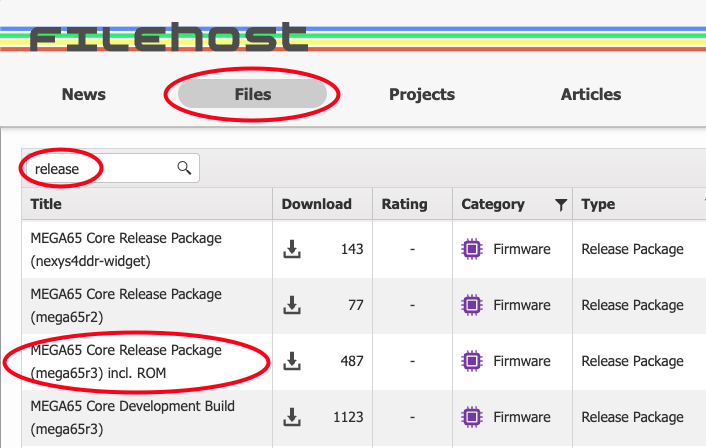
\includegraphics[width=0.7\linewidth]{images/filehost_release.png}}
\end{center}

Extract the downloaded {\tt .7z} archive. You should see a file whose name ends in {\tt .cor}, and a folder of {\tt sdcard-files} that includes one named {\tt MEGA65.ROM}.

\section{The Core Selection Menu}
\index{Core!Core Selection Menu}

The MEGA65 decides which core to load into the FPGA when it starts up. You can interrupt this process to select which core to load.\footnote{Technically, the MEGA65 starts the core in slot 0 to power the core selection menu. After you have made a selection or it chooses a default, it loads the selected core into the FPGA and continues the boot process.}

To open the core selection menu, switch off the computer, then hold the \specialkey{NO\\SCROLL} key and switch on the computer. The core selection menu appears, with the eight core slots numbered 0 through 7.

\begin{center}
  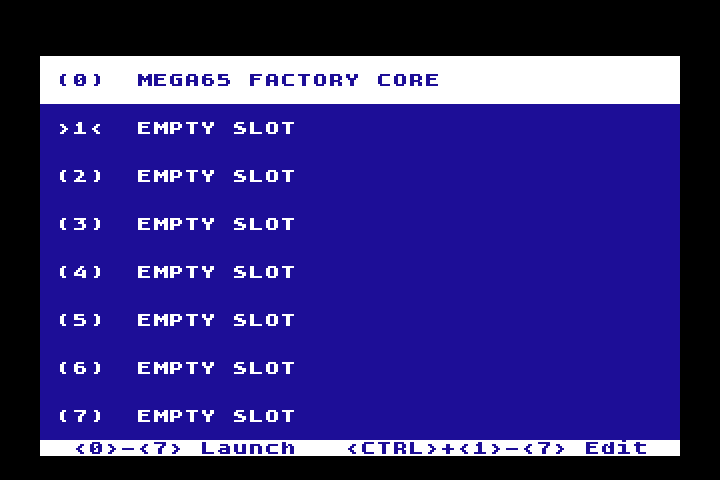
\includegraphics[width=0.7\linewidth]{images/ss-flashmenu.png}
\end{center}

You can select a core to boot using the cursor keys and \specialkey{RETURN}, or you can simply press the number key that corresponds to the slot. The boot process continues with the new core. The MEGA65 will keep running the new core until you switch it off. (Pressing the reset button will not reset which core is being run.)

When you switch on the computer without opening the core selection menu, the MEGA65 looks for a default core. It first checks to see if any core is flagged as the default core (a setting you can change). If none are flagged, then it checks to see if there is a core in slot 1.\footnote{If DIP switch \#4 is in the ``on'' position, the MEGA65 checks slot 2 instead of slot 1. DIP switches are located inside the case, on the main board.} If the slot is empty, it uses slot 0.

Your computer comes with the MEGA65 core in slot 0 installed at the factory. It is recommended that you do not upgrade the factory-installed core unless advised to do so by the MEGA65 team. Instead, install new versions of the MEGA65 core in slot 1.

\section{Upgrading the MEGA65 Core, ROM, and System Files}
\index{Core!Upgrading}\index{ROM!Upgrading}

You can upgrade a core, or install a new core, from the core selection menu. This process reads the {\tt .cor} file from the SD card.

To upgrade the MEGA65 core, ROM, and system files:

\begin{enumerate}
  \item Remove the SD card (or microSD card) from the MEGA65, and connect it to your PC using an SD card reader.\footnote{As an alternative to moving the SD card to your PC, you can transfer files using an Ethernet connection. See chapter \vref{cha:transferring-files}.}
  \item Copy the {\tt .cor} file that you extracted from the {\tt .7z} archive to the SD card.
  \item On your PC, open the {\tt sdcard-files} folder from the {\tt .7z} archive, then copy those files to the SD card, replacing the existing files. Put them in the root of the SD card's file system, not a sub-folder.
  \item Eject the SD card from your PC's operating system, then move it back to the MEGA65.
  \item Open the core selection menu: switch off the MEGA65, then hold \specialkey{NO\\SCROLL} while switching it back on.
  \item Hold \specialkey{CTRL} then press the number of the slot you want to upgrade. The slot editor opens.
  \item Press \specialkey{F3} to load a core file. The file selector opens. Use the cursor keys to select the {\tt .cor} file, then press \specialkey{RETURN}.
  \item Press \specialkey{F8} to flash the core slot. Allow the flashing process to complete. This takes several minutes.
  \item When the flashing process is complete, press any key to return to the core selection menu.
\end{enumerate}

The slot editor looks like this:

\begin{center}
  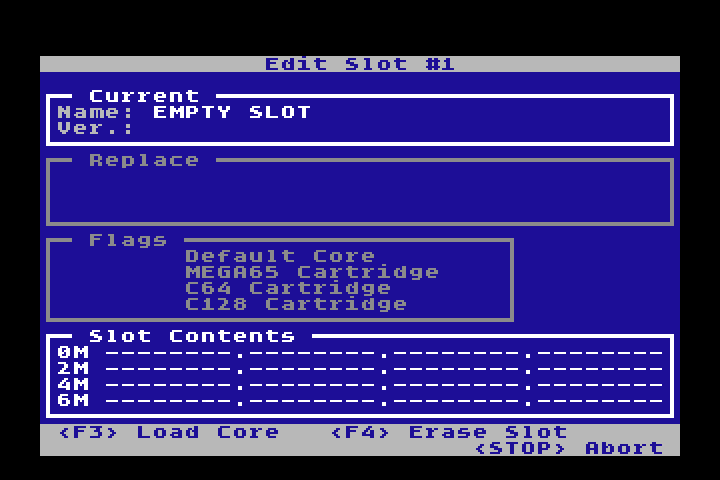
\includegraphics[width=0.7\linewidth]{images/ss-flashmenu-sloteditor.png}
\end{center}

When you load a core file, it prompts you to select the {\tt .cor} file on a screen that looks similar to this:

\begin{center}
  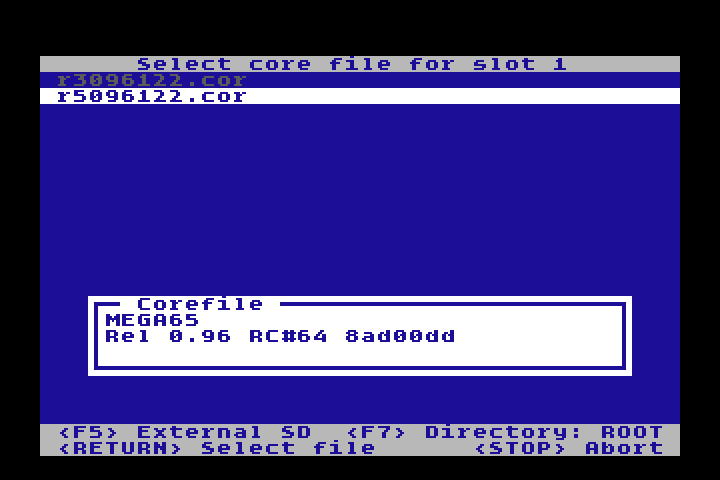
\includegraphics[width=0.7\linewidth]{images/ss-flashmenu-selectcore.png}
\end{center}

Once you have selected the core, the slot editor shows the change it intends to make to the slot. After you start the flashing process, the display shows the progress.

\underline{NOTE}: Do {\em not} switch off your computer or disconnect power until after this step is complete.

\begin{center}
  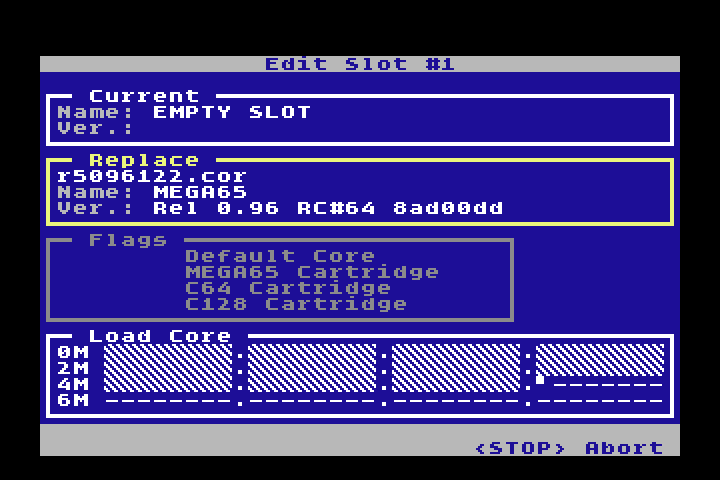
\includegraphics[width=0.7\linewidth]{images/ss-flashmenu-loading.png}
\end{center}

When the message "Core was successfully flashed" is displayed, the process is complete.

\begin{center}
  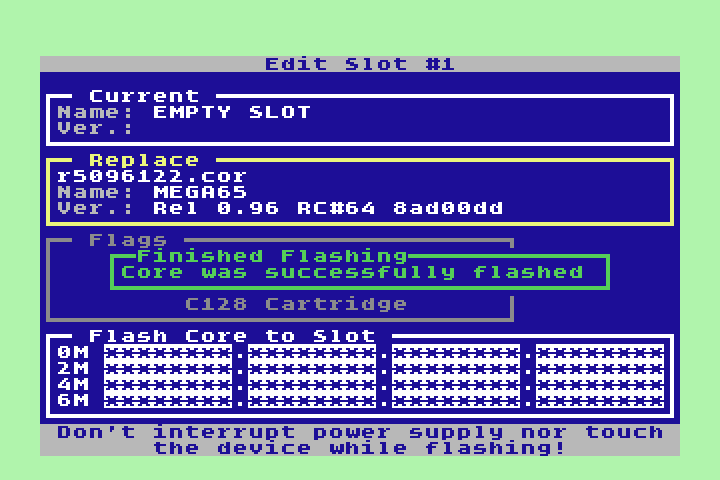
\includegraphics[width=0.7\linewidth]{images/ss-flashmenu-complete.png}
\end{center}

It is now safe to switch off your computer. Press any key to return to the core selection menu, or switch the computer off then on again to start the default core.


\section{Installing Alternate Cores and ROMs}

Installing an alternate core, such as the C64 core,\index{Core!C64 core} uses the same steps for flashing the core to a slot.

It is recommended to use slots 2 through 7 for alternate cores, and reserve slot 1 for the latest MEGA65 core. Of course, there is nothing stopping you from installing an alternate core in slot 1, so that the MEGA65 behaves as a different type of computer when you switch it on. You can always choose the MEGA65 core from the core selection menu.

You can keep more than one version of the MEGA65 ROM on the SD card. When booting the MEGA65 core, you can select one of these ROMs by holding down a number key during boot.

To install alternate ROMs, copy them to the root of the SD card with a filename such as {\tt MEGA65x.ROM}, where {\tt x} is a number between 1 and 7. To boot the alternate ROM, hold the corresponding number key down while the MEGA65 core starts. If you do not hold down a number, it boots to {\tt MEGA65.ROM} by default.

There are several reasons you might want to keep alternate ROMs on your SD card:

\begin{itemize}
  \item You are helping to test a new beta release of the ROM, and do not wish to make the beta version your default ROM.
  \item You want to try the original Commodore 65 prototype ROM. The MEGA65 core maintains backwards compatibility with the C65 ROM that was in progress by Commodore before they cancelled the project. It is buggy and incomplete, but is still an interesting historical artifact.
  \item You want to try an alternate ROM developed by the MEGA65 community. One such ROM is the MEGA65 OpenROM, a project to create an all-new ROM released under an Open Source license without any original Commodore material.
\end{itemize}

Several alternate ROMs came with your MEGA65 SD card, installed at the factory. Try rebooting your computer while holding down a number key to see what happens!

\section{Setting Core Flags}

There are several options ("flags") that you can select for a core in the core editor. Press the number key that corresponds to the flag to toggle its value.

To set the core to be the default core used when the MEGA65 is switched on without \specialkey{NO\\SCROLL} held down, set the "Default core" flag. If no core is set as the default core, then slot 1 is used as the default (or slot 2 if DIP switch \#4 is set to on).

The "cartridge" flags determine which core is selected when a cartridge is present in the expansion slot. This allows you to choose a different default core based on the type of the cartridge. For example, you can set the MEGA65 core to handle MEGA65 cartridges, and a different core to handle C64 cartridges. By default, the MEGA65 core will handle C64 cartridges using "GO64" mode. You may prefer to change this to use the C64 core that you install separately.

\begin{center}
  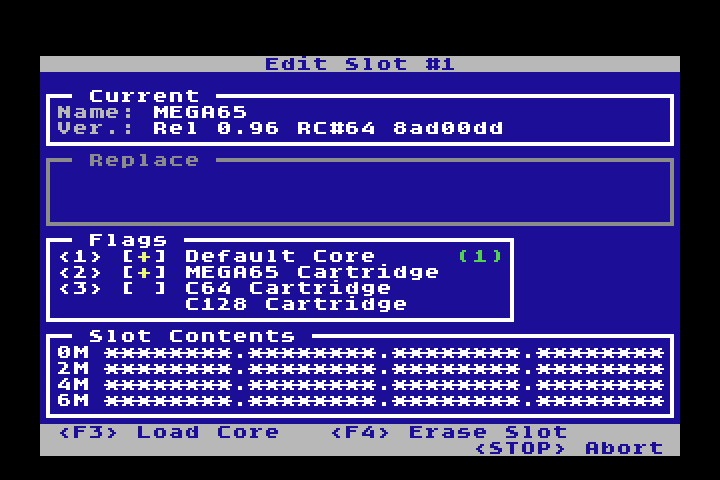
\includegraphics[width=0.7\linewidth]{images/ss-flashmenu-flags.png}
\end{center}

\section{Erasing a Core Slot}

The flashing process replaces whatever is in a core slot with the new core. If a core is already installed in the slot, flashing overwrites the existing core.

If you wish to delete a core and leave the slot empty, edit the slot, press \specialkey{F4} to set the replacement to "Erase slot," then press \specialkey{F8} to flash the slot with empty data.

\section{Upgrading the Factory Core in Slot 0}
\index{Core!Upgrading Slot 0}

It is possible to upgrade the factory-installed MEGA65 core in slot 0. You only need to do this in rare cases, such as if a newer version of the MEGA65 core includes changes or bug fixes for the start-up process. It is recommended that you do not upgrade slot 0 unless the announcement for the release suggests that you do so. Most MEGA65 core upgrades are fully functional in slot 1, without needing to upgrade slot 0.

It is important that at least one core slot contains a functioning MEGA65 core. If something goes wrong during the flashing process, this may result in a non-functioning core in that slot. To help prevent accidents, the procedure for flashing slot 0 is slightly different from that of the other slots, and only an official MEGA65 core can be flashed to slot 0.

{\em Please read these instructions carefully before starting the procedure.} To upgrade the core in slot 0:

\begin{enumerate}
  \item Install the latest MEGA65 core in slot 1, using the procedure described earlier. The core must be in the default non-zero slot to recover from any problems when updating slot 0.
  \item Launch core slot 1 to confirm that it works.
  \item Open the core selection menu. Hold the \megasymbolkey and press the comma key to open the editor for slot 0.
  \item Repeat the remainder of the flashing procedure to select the core file and flash the slot.
\end{enumerate}

\ifdefined\printmanual
\else
\underline{NOTE}: If you have a revision R3A MEGA65 and have not previously upgraded slot 0, the \megasymbolkey and the comma key will not start the procedure: you have an older slot 0 core that does not have this feature. You can work around this by restarting the core selection menu with slot 1. From the core selection menu, prepare to hold down \specialkey{NO\\SCROLL}, press the \megakey{1} key to boot into the core then immediately press and hold \specialkey{NO\\SCROLL}. The core selection menu re-opens using slot 1. Press \megasymbolkey and the comma key to complete the slot 0 upgrade.
\fi

If something goes wrong during the slot 0 flashing process, your MEGA65 may not start correctly. Before doing anything else, switch on your MEGA65, and wait a minute or so. After a while, it should notice that there is no valid core in slot 0, then proceed to start the core in slot 1. You can hold \specialkey{NO\\SCROLL} during this to open slot 1's core selection menu and restart the flashing process.

If the MEGA65 cannot boot any core after several minutes, it may be stuck. You may be able to recover using a device known as a ``JTAG interface'' that connects your PC to the MEGA65 main board. This allows you to inject a bitstream directly into the FPGA. The part is inexpensive but not always available. Contact the MEGA65 team on the Discord (\url{https://mega65.org/chat}) for assistance.

Core slot 0 cannot be assigned flags, such as to be the default core or to be associated with cartridge types. It will be used for these purposes if no other core is installed. It is recommended that you keep the latest MEGA65 core in slot 1, in addition to flashing slot 0.


\section{Understanding The Core Booting Process}
\nopagebreak
This section summarises how the MEGA65 selects which core to start with when it is switched on. The process is shown in the following figure:
\nopagebreak
\includegraphics[width=\linewidth]{images/illustrations/flashmenu-flowchart.pdf}

The booting process is governed by two facilities:
\begin{itemize}
  \item The Hypervisor (also known as HYPPO), which operates at a level above the KERNAL. One of its responsibilities is to manage aspects of the boot process. For more details on the Hypervisor, refer to
\ifdefined\printmanual
the {\bf MEGA65 Book}.
\else
 \bookvref{sec:hypervisor-mode}.
\fi
    In the diagram, activities performed by the Hypervisor have been highlighted in green.
  \item The Core Selection Menu program (also known as ``MegaFlash''), which provides a list of available core slots to choose from. In the diagram, activities performed by MegaFlash have been highlighted in blue.
\end{itemize}

When the MEGA65 is switched on, it does the following:
\begin{itemize}
\item Loads the bitstream stored in slot 0 of flash memory. If that is the MEGA65 Factory Core, the MEGA65
  HYPPO Hypervisor starts.
\item If it is the first boot since power-on (which implies that you are running from slot 0), HYPPO starts the Flash Menu program (aka MegaFlash) -- but note that the Flash Menu in
      this mode may not show anything on the screen to indicate that it is running!
\item The Flash Menu then checks if \specialkey{NO\\SCROLL} is being held down.
\item If it is, the Flash Menu program shows its display, allowing you to select or re-flash a core.
\item If \specialkey{NO\\SCROLL} is {\em not} being held down, the Flash Menu program checks if Flash Slot 1 contains a valid
      core.
\item If it does, then the Flash Menu program attempts to load that core.
\item If it succeeds, then the system reconfigures itself for that core, after which the behaviour of the system is
      according to that core.
\item If it fails, the keyboard will go into ``ambulance mode'', showing flashing blue lights to indicate that some
      first-aid is required. Note that in ambulance mode the reset button has no effect: You must switch the
      MEGA65 off and on again.
\end{itemize}

If you have selected a different core in the Core Selection Menu, the process is similar, except that the ambulance lights will appear for only a limited time, as the FPGA will automatically search through the flash memory until it finds a valid core. If it gets to the end of the flash memory, it will start the MEGA65 Factory Core from slot 0 again.
